\documentclass[11pt,a4paper]{article}

% package importing
%\usepackage[margin=2cm]{geometry}
\usepackage{geometry}
 \geometry{
 a4paper,
 %total={170mm,257mm},
 left=20mm,
 top=20mm,
 right=20mm,
 bottom=20mm,
 }
 		%$$$$$$ fonts settings $$$$$$%
%\usepackage[sc]{mathpazo}  %for palatino font
%\usepackage{eulervm}  %for Euler maths font

		%$$$$$$ package imports $$$$$$%
\usepackage{amsmath}  %for mathematics
\usepackage{titlesec}  %for title spacing only
\usepackage{lipsum}  %random huge text generation
\usepackage{titlesec} %for changing font of titles 
\usepackage{amssymb}  %for real number set symbol
\usepackage{amsthm}  %for mathematics package
\usepackage{mathtools}  %for floor and ceiling
\usepackage{algorithmicx}  %for dynamic algorithm
\usepackage{algorithm}  %algorithm micro
\usepackage{algpseudocode}  %pseudocode commands
\usepackage{wrapfig}  %for wrapping figures around text
\usepackage{multicol}  %for multiple columns floats
\usepackage{enumitem}  %for enumerate numbering
\usepackage{url}   %for writing the url
\usepackage{color}  %for colorred text
\usepackage{tcolorbox}  %for colour box highlighting
\usepackage{listings}  %for code listing

% $$$$$$$$$ new command and theorems self-defined
\theoremstyle{definition}
\newtheorem{theorem}{Theorem}[section]
\newtheorem{corollary}{Corollary}[theorem]
\newtheorem{lemma}[theorem]{Lemma}
\newtheorem*{remark}{Remark}
\newtheorem{definition}{Definition}[section]
\newtheorem{example}{Example}[section]
\newtheorem{notation}{Notation}[section]
\newtheorem{algoalgorithm}{Algorithm}[section]
\newtheorem{method}{Method}[section]

% $$$$$$$$ set general info $$$$$$$
\title{\textsl{National University of Singapore} \\ \textbf{CS2106 Operating System}\\ Second Half Summary Notes}
\author{\textit{Dong Shaocong} A0148008J}

% $$$$$$$$ package parameter setting $$$$$$$$$

% for title spacing {left}{before}{after}  ----------------------------
\titlespacing\section{0.5pt}{10pt plus 2pt minus 2pt}{2pt plus 2pt minus 1pt}
\titlespacing\subsection{0.5pt}{10pt plus 2pt minus 2pt}{2pt plus 2pt minus 1pt}
\titlespacing\subsubsection{0.5pt}{10pt plus 2pt minus 2pt}{2pt plus 2pt minus 1pt}

% for title font specifications  ------------------------------------------
\titleformat{\section}
  {\normalfont\fontsize{16}{16}\bfseries}
  {\thesection}{1em}{}
  
\titleformat{\subsection}
  {\normalfont\fontsize{14}{14}\bfseries}{\thesection}{1em}{}
  
\titleformat{\subsubsection}
  {\normalfont\fontsize{13}{13}\bfseries}{\thesection}{1em}{}

% declare floor and ceiling functions   ------------------------------------------
\DeclarePairedDelimiter\ceil{\lceil}{\rceil}
\DeclarePairedDelimiter\floor{\lfloor}{\rfloor}

% set the numbering of enumerate to numbers------------------------------------------
\setlist[enumerate]{label*=\arabic*.}
%\setlist{nolistsep}
\newenvironment{myitemize}
{ \begin{itemize}
    \setlength{\itemsep}{5pt}
    \setlength{\parskip}{0pt}
    \setlength{\parsep}{0pt}     }
{ \end{itemize}                  } 
\newenvironment{myenumerate}
{ \begin{enumerate}
    \setlength{\itemsep}{5pt}
    \setlength{\parskip}{0pt}
    \setlength{\parsep}{0pt}     }
{ \end{enumerate}                } 

% $$$$$$$$$ math symbols cheatsheet
% Caligraphic letters: $\mathcal{A}$ 
% Mathbb letters: $\mathbb{A}$
% Mathfrak letters: $\mathfrak{A}$ 
% Math Sans serif letters: $\mathsf{A}$ 
% $$$$$ color text commands ------------
\newcommand{\redtt}[1]{{\color{red}\texttt{#1}}}
\newcommand{\bluett}[1]{{\color{blue}\texttt{#1}}}
\newcommand{\browntt}[1]{{\color{brown}\texttt{#1}}}
\newcommand{\bluebf}[1]{{\color{blue} \huge \textbf{#1}}}
\renewcommand{\emph}[2]{\redtt{#1} \bluebf{#2}}
%-------------------------------------------------------

% $$$$$$$$ start of documents $$$$$$$$$
\begin{document}
\maketitle
\section{File System}

\begin{definition}{\textbf{File system}}
	\begin{myitemize}
		\item Present logical (abstract) view of files and directories
		\begin{myitemize}
			\item Accessing a disk is very complicated: (2D or 3D structure, track/surface/sector, seek, rotation, $\dots$)
			\item Hide complexity of hardware devices
		\end{myitemize}
		\item Facilitate efficient use of storage devices: Optimise access e.g. to disk.
		\item Support sharing
		\begin{myitemize}
			\item Files persist even when owner/creator is not currently active (unlike main memory)
			\item Key issue: Provide protection (control access)
		\end{myitemize}
	\end{myitemize}
\end{definition}

\begin{definition}{\textbf{Hierarchical View of File system}}
	\begin{center}
		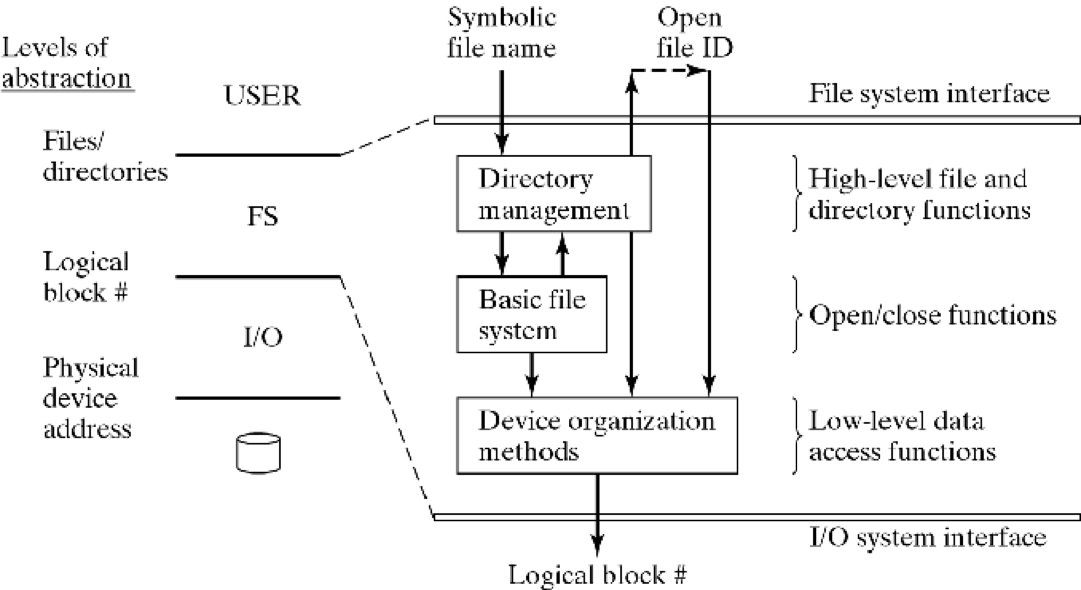
\includegraphics[scale=0.5]{m2/hierarchyFileSystem}
	\end{center}
	\begin{myitemize}
		\item \textbf{Directory management}: map logical name to
unique Id, file descriptor
		\item \textbf{Basic file system}: open/close files
		\item \textbf{Physical device  organization}: map file data to disk blocks
	\end{myitemize}
\end{definition}

\begin{definition}{\textbf{User-end view of File}}
	\begin{myitemize}
		\item \textbf{File name and type}
		\begin{myitemize}
			\item Valid name: number or characters, lower or upper cases, illegal characters $\dots$
			\item Extension: tied to type of file, used by applications
			\item File type is recorded in header
			\begin{myitemize}
				\item Cannot be changed (even when extension changes)
				\item Basic types: text, object, load file, directory
				\item  
			\end{myitemize}
		\end{myitemize}
	\end{myitemize}
\end{definition}


% $$$$$$$$$$$$$$$$$$$$$$$$$$$$$$$$$$ %
\newpage
\begin{myitemize}
	\item 
\end{myitemize}

{\color{red} red } \textsf{sftext} \texttt{tttext}
\begin{tcolorbox} 
Penghao is the best \LaTeX \, writer.
\end{tcolorbox}
\begin{tcolorbox}
	\begin{lstlisting}
		def func():
			print("Penghao is cool!")
	\end{lstlisting}
\end{tcolorbox}
\noindent{}\\\noindent$\wp\wp\wp\wp\wp\wp\wp\wp\wp\wp\wp\wp\wp\wp\wp\wp\wp\wp\wp\wp\wp\wp\wp\wp\wp\wp\wp\wp\wp\wp\wp\wp\wp\wp\wp$\\
{}\\
\lipsum[1]

% ---- important examples ----%
\vspace{-\topsep}
\begin{enumerate}
	\item 123
	\item 123
	\item 123
\end{enumerate}
\vspace{-\topsep}

\begin{center}
 \begin{tabular}{|| c || c | c | c |c |c ||} 
 \hline
  & M1 & M2 & M3 & M4 & M5 \\ [0.5ex] 
 \hline\hline
 M1 & 0 & 108 & 180 & 228 & 396 \\ 
 \hline
 M2 &  & 0 & 72 & 168 & 288 \\
 \hline
 M3 &  &  & 0 & 48 & 144 \\
 \hline
 M4 &  &  &  & 0 & 128 \\
 \hline
 M5 &  &  & &  & 0   \\ [0.5ex] 
 \hline
\end{tabular}
\end{center}

\begin{algorithm}
\caption{title}
%\begin{multicols}{2}
\begin{algorithmic}[1]
\State 123
\end{algorithmic}
%\end{multicols}
\end{algorithm}

\begin{thebibliography}{9}
 
\bibitem{einstein} 
Albert Einstein. 
\textit{Zur Elektrodynamik bewegter K{\"o}rper}. (German) 
[\textit{On the electrodynamics of moving bodies} \url{www.google.com.sg}]. 
Annalen der Physik, 322(10):891–921, 1905.
\end{thebibliography}

\end{document}